\documentclass[tikz]{standalone}

\begin{document}
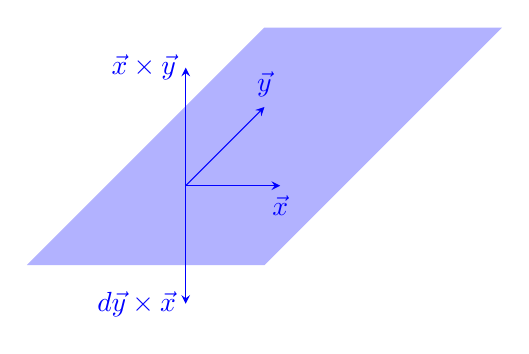
\begin{tikzpicture}
  \draw[blue!30,fill=blue!30] (-2,-1) -- (1,-1) -- (4,2) -- (1,2) -- cycle;	
  \draw[blue,->,>=stealth] (0,0) -- (1,1) node[above] {\(\vec{y}\)};
  \draw[blue,->,>=stealth] (0,0) -- (1.2,0) node[below] {\(\vec{x}\)};	
  \draw[blue,->,>=stealth] (0,0) -- (0,1.5) node[left] {\(\vec{x}\times \vec{y}\)};
  \draw[blue,->,>=stealth] (0,0) -- (0,-1.5) node[left] {\(d\vec{y}\times \vec{x}\)};
\end{tikzpicture}
\end{document}
